\section{Aufbau und Durchf"uhrung}
	\label{sec:durchfuehrung}

	Um das Emissionsverm"ogen zu bestimmen, kann die abgetrahlte Leistung eines K"orpers gemessen werden.
	Der gesuchte Wert $\epsilon$ ergibt sich dann aus einer linearen Regression aus den Messwerten in der Gleichung \eqref{boltzmann}.

	\begin{figure}[h!]
		\centering
		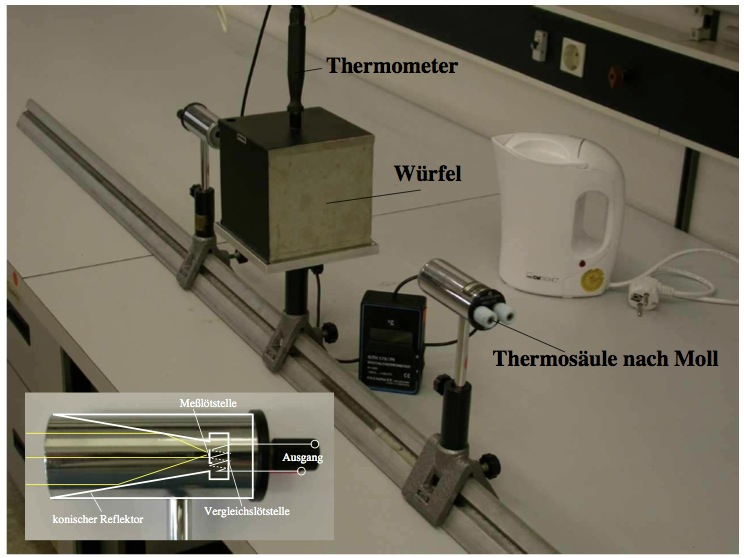
\includegraphics[width = 15cm]{img/aufbau.JPG}
		\caption{Versuchsaufbau}
		\label{fig:aufbau}
	\end{figure}

	In diesem Versuch wird ein W"urfel mit kochendem Wasser bef"ullt.
	Vier Seiten des W"urfels bestehen aus verschiedenen Materialien, wodurch jeweils ein K"orper mit unterschiedlichen Emissionsverm"ogen simuliert wird.
	Einen solchen W"urfel nennt man auch Leslie-W"urfel.

	Ein Teil der abgestrahlten Leistung $P$ wird mit Hilfe einer Thermos"aule nach Moll gemessen.

	Dieses Ger"at liefert durch ein Thermoelement eine Spannung, die proportional zur ab\-ge\-strahl\-ten W"arme der gegen"uberliegenden Oberfl"ache ist.
	Das Thermoelement ist durch einen Zylinder mit kegelf"ormiger "Offnung umgeben.
	Es ist darauf zu achten, dass das Geh"ause nicht ber"uhrt wird, da die Referenztemperatur des Thermoelements in diesem gemessen wird und schon kleine Schwankungen die Messwerte verf"alschen.

	Abbildung \ref{fig:aufbau} zeigt den Versuchsaufbau.


	Schlie"slich wird die Leistung $P$ in wachsendem Abstand $r$ gemessen und die Messwerte visualisiert.
	Weil es sich bei der Strahlung um Kugelwellen handelt, ist eine $1 / r^2$ Abh"angigkeit zu erwarten.